\documentclass{article}

\def\npart {II}
\def\nyear {2017}
\def\nterm {Lent}
\def\nlecturer{Dr R.\ Camina}
\def\ncourse{Coding and Cryptography}
\def\draft{Rough}
\ifx \nauthor\undefined
  \def\nauthor{Bhavik Mehta}
\else
\fi

\author{Based on lectures by \nlecturer \\\small Notes taken by \nauthor}
\date{\nterm\ \nyear}
\title{Part \npart\ -- \ncourse}

\usepackage[utf8]{inputenc}
\usepackage{amsmath}
\usepackage{amsthm}
\usepackage{amssymb}
\usepackage{enumerate}
\usepackage{mathtools}
\usepackage{graphicx}
\usepackage[dvipsnames]{xcolor}
\usepackage{tikz}
\usepackage{wrapfig}
\usepackage{centernot}
\usepackage{float}
\usepackage{braket}
\usepackage[hypcap=true]{caption}
\usepackage{enumitem}
\usepackage[colorlinks=true, linkcolor=mblue]{hyperref}
\usepackage[nameinlink,noabbrev]{cleveref}
\usepackage{nameref}
\usepackage[margin=1.5in]{geometry}

% Theorems
\theoremstyle{definition}
\newtheorem*{aim}{Aim}
\newtheorem*{axiom}{Axiom}
\newtheorem*{claim}{Claim}
\newtheorem*{cor}{Corollary}
\newtheorem*{conjecture}{Conjecture}
\newtheorem*{defi}{Definition}
\newtheorem*{eg}{Example}
\newtheorem*{ex}{Exercise}
\newtheorem*{fact}{Fact}
\newtheorem*{law}{Law}
\newtheorem*{lemma}{Lemma}
\newtheorem*{notation}{Notation}
\newtheorem*{prop}{Proposition}
\newtheorem*{question}{Question}
\newtheorem*{rrule}{Rule}
\newtheorem*{thm}{Theorem}
\newtheorem*{assumption}{Assumption}

\newtheorem*{remark}{Remark}
\newtheorem*{warning}{Warning}
\newtheorem*{exercise}{Exercise}

% \newcommand{\nthmautorefname}{Theorem}

\newtheorem{nthm}{Theorem}[section]
\newtheorem{nlemma}[nthm]{Lemma}
\newtheorem{nprop}[nthm]{Proposition}
\newtheorem{ncor}[nthm]{Corollary}
\newtheorem{ndef}[nthm]{Definition}

% Special sets
\newcommand{\C}{\mathbb{C}}
\newcommand{\N}{\mathbb{N}}
\newcommand{\Q}{\mathbb{Q}}
\newcommand{\R}{\mathbb{R}}
\newcommand{\Z}{\mathbb{Z}}

\newcommand{\abs}[1]{\left\lvert #1\right\rvert}
\newcommand{\norm}[1]{\left\lVert #1\right\rVert}
\renewcommand{\vec}[1]{\boldsymbol{\mathbf{#1}}}

\let\Im\relax
\let\Re\relax

\DeclareMathOperator{\Im}{Im}
\DeclareMathOperator{\Re}{Re}
\DeclareMathOperator{\id}{id}

\definecolor{mblue}{rgb}{0., 0.05, 0.6}


% preamble
\usepackage{tikz}
\usepackage{pgfplots}
\usepackage{tikz-cd}
\usepackage{extarrows}
\usepackage{bm}
\usetikzlibrary{arrows,decorations.pathmorphing,decorations.markings,positioning}
% \renewcommand{\thesection}{\Roman{section}}
\DeclarePairedDelimiter{\floor}{\lfloor}{\rfloor}
\DeclarePairedDelimiter{\ceil}{\lceil}{\rceil}
\pgfplotsset{width=7cm}
\newcommand{\barP}{\mid}
\newcommand{\probConv}{\hyperlink{def:probConverge}{\xlongrightarrow{p}}}
\newcommand{\Prob}{\mathbb{P}}
\newcommand{\Exp}{\mathbb{E}}
% and here we go!

\begin{document}
\maketitle
\tableofcontents

\clearpage
\section*{Introduction to communication channels and coding}
For example, given a message $m$=`Call me!' which we wish to send by email, first encode as binary strings using ASCII.
So, $f(C) = 1000011, f(a) = 1100001$, and $f^*(m) = 1000011\ 1100001 \dots 0100001$.
% picture
\tikzstyle{block} = [rectangle, draw, fill=YellowOrange!20,
    text width=4em,
    text centered,
    minimum height=2em
    ]
\begin{center}
    \begin{tikzpicture}[node distance=3cm]
        \node (s) at (0, 0) [block] {source};
        % this is kind of horrible but it works :/
        \node (e) at (3, 0) [block] {encoder};
        \node (d) at (8, 0) [block] {decoder};
        \node (r) at (11, 0) [block] {receiver};
        \draw [->, shorten > =0.1em, thick] (s) -- (e);
        \draw [->, shorten > =0.1em, thick, decorate, decoration={amplitude=1.5mm,
            segment length=10mm,
            snake, post length=1mm}] (e) -- (d)
            node [above=0.5em,align=center,midway] {channel}
            node [below=0.5em,align=center,midway,color=red] {errors};

        \draw [->, shorten > =0.1em, thick] (d) -- (r);
    \end{tikzpicture}
\end{center}

\textbf{Basic problem:} Given a source and a channel (described probabilistically) we aim to design an encoder and a decoder in order to transmit information both \emph{economically} and \emph{reliably} (coding) and maybe also to \emph{preserve privacy} (cryptography).

\begin{eg}
\leavevmode
\begin{itemize}[label={--}]
    \item `Economically': In Morse code, common letters have shorter codewords:
    \begin{equation*}
        A = \text{.-} \quad E = \text{.} \quad Q = \text{-{}-.-}
    \end{equation*}
    \item `Reliably': Every book has an ISBN of form $a_1 a_2 \dotsc a_{10}$ where $a_i \in \{0, 1, \dotsc, 9\}$ for $1 \leq i \leq 9$, $a_{10} \in \{0, 1, \dotsc, 9, X\}$ such that
    \begin{equation*}
        10 a_1 + 9 a_2 + \dotsc + a_{10} \equiv 0 \pmod{11}
    \end{equation*}
    so errors can be detected (but not corrected).
    Similarly a 13-digit ISBN has
    \begin{equation*}
        x_1 + 3 x_2 + x_3 + 3 x_4 + \dotsc + 3 x_{12} + x_{13} \equiv 0 \pmod{10}
    \end{equation*}
    for $0 \leq x_i \leq 10$, doesn't necessarily spot transpositions.
    \item `Preserve privacy' e.g. RSA.
\end{itemize}
\end{eg}

A \textbf{communication channel} takes letters from an input alphabet $\Sigma_1 = \{a_1, \dotsc, a_r\}$ and emits letters form an output alphabet $\Sigma_2 = \{b_1, \dotsc, b_s\}$.

A channel is determined by the probabilities
\begin{equation*}
    \Prob(y_1 \dotsc y_k \text{ received} \mid x_1 \dotsc x_k \text{ sent})
\end{equation*}

\begin{defi}[Discrete memoryless channel]\hypertarget{def:dmc}
    A \textbf{discrete memoryless channel} (DMC) is a channel for which
    \begin{equation*}
        P_{ij} = \Prob(b_j \text{ received} \mid a_i \text{ sent})
    \end{equation*}
    is the same each time the channel is used and is independent of all past and future uses.
\end{defi}

The channel matrix is the $r \times s$ matrix with entries $p_{ij}$ (note the rows sum to 1).

\begin{eg}
    Binary Symmetric Channel \hypertarget{def:bsc}{(BSC)} has $\Sigma_1 = \Sigma_2 = \{0, 1\}$, $0 \leq p \leq 1$:
    \begin{center}
        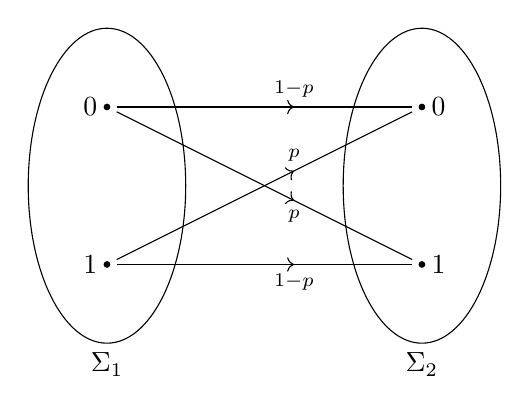
\begin{tikzpicture}
            \draw (-2, 0) circle [x radius=1cm, y radius=2cm] node [below=2cm] {$\Sigma_1$};
            \draw ( 2, 0) circle [x radius=1cm, y radius=2cm] node [below=2cm] {$\Sigma_2$};

            \node (0l) at (-2, 1) {};
            \node (1l) at (-2,-1) {};

            \node (0r) at (2, 1) {};
            \node (1r) at (2,-1) {};

            \filldraw (0l) circle (1pt) node [left] {0};
            \filldraw (1l) circle (1pt) node [left] {1};
            \filldraw (0r) circle (1pt) node [right] {0};
            \filldraw (1r) circle (1pt) node [right] {1};

            \begin{scope}[decoration={
                markings,
                mark=at position 0.6 with {\arrow{>}}}
                ]
                \draw[postaction={decorate}] (0l) -- (0r)
                    node [above,align=center,pos=0.6] {$\scriptstyle 1-p$};
                \draw[postaction={decorate}] (0l) -- (1r)
                    node [below,align=center,pos=0.6] {$\scriptstyle p$};
                \draw[postaction={decorate}] (1l) -- (0r)
                    node [above,align=center,pos=0.6] {$\scriptstyle p$};
                \draw[postaction={decorate}] (1l) -- (1r)
                    node [below,align=center,pos=0.6] {$\scriptstyle 1-p$};
            \end{scope}
        \end{tikzpicture}
    \end{center}
    with channel matrix
    \begin{equation*}
        \begin{pmatrix}
            1-p & p \\ p & 1-p
        \end{pmatrix}
    \end{equation*}
    i.e. $p$ is the probability a symbol is mistransmitted.


    Another example is given by the Binary Erasure channel, $\Sigma_1 \{0, 1\}$, $\Sigma_2 = \{0, 1, *\}$ and $0 \leq p \leq 1$.
    \begin{center}
        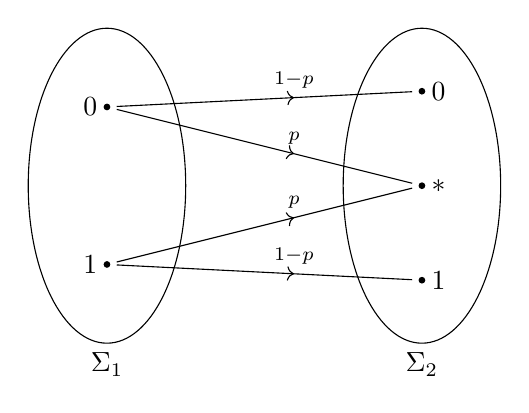
\begin{tikzpicture}
            \draw (-2, 0) circle [x radius=1cm, y radius=2cm] node [below=2cm] {$\Sigma_1$};
            \draw ( 2, 0) circle [x radius=1cm, y radius=2cm] node [below=2cm] {$\Sigma_2$};

            \node (0l) at (-2, 1) {};
            \node (1l) at (-2,-1) {};

            \node (0r) at (2, 1.2) {};
            \node (*r) at (2,   0) {};
            \node (1r) at (2,-1.2) {};

            \filldraw (0l) circle (1pt) node [left] {0};
            \filldraw (1l) circle (1pt) node [left] {1};
            \filldraw (0r) circle (1pt) node [right] {0};
            \filldraw (*r) circle (1pt) node [right] {$*$};
            \filldraw (1r) circle (1pt) node [right] {1};

            \begin{scope}[decoration={
                markings,
                mark=at position 0.6 with {\arrow{>}}}
                ]
                \draw[postaction={decorate}] (0l) -- (0r)
                    node [above,align=center,pos=0.6] {$\scriptstyle 1-p$};
                \draw[postaction={decorate}] (0l) -- (*r)
                    node [above,align=center,pos=0.6] {$\scriptstyle p$};
                \draw[postaction={decorate}] (1l) -- (*r)
                    node [above,align=center,pos=0.6] {$\scriptstyle p$};
                \draw[postaction={decorate}] (1l) -- (1r)
                    node [above,align=center,pos=0.6] {$\scriptstyle 1-p$};
            \end{scope}
        \end{tikzpicture}
    \end{center}
    with channel matrix
    \begin{equation*}
        \begin{pmatrix}
            1-p & p & 0 \\
            0 & p & 1-p
        \end{pmatrix}
    \end{equation*}
    i.e. $p$ is the probability a symbol can't be read.
\end{eg}

Informally, a channel's capacity is the highest rate at which information can be reliably transmitted over the channel.
Rate refers to units of information per unit time, which we want to be high. Similarly, reliably means we want an arbitrarily small error probability.

\clearpage
\section{Noiseless Coding}
\begin{notation}
    For $\Sigma$ an alphabet, let $\Sigma^* = \bigcup_{n \geq 0} \Sigma^n$ be the set of all finite strings of elements of $\Sigma$.
\end{notation}
If $x = x_1 \dotsc x_r$, $y = y_1 \dotsc y_s$ are strings from $\Sigma$, write $xy$ for the concatenation $x_1 \dotsc x_r y_1 \dotsc y_s$.
Further, $\abs{x_1 \dotsc x_r y_1 \dotsc y_s} = r+s$, the length of the string.
\begin{defi}[Code]\hypertarget{def:code}
    Let $\Sigma_1, \Sigma_2$ be two alphabets. A \textbf{code} is a function $f: \Sigma_1 \to \Sigma_2^*$. The strings $f(x)$ for $x \in \Sigma_1$ are called \textbf{codewords}.
\end{defi}
\begin{eg}
    \leavevmode
    \begin{enumerate}[label=\arabic*)] % 1)
        \item
            \hypertarget{ex:greekFire}{Greek fire} \hyperlink{def:code}{code}:
            \begin{align*}
                \Sigma_1 &= \{\alpha, \beta, \gamma, \dotsc, \omega\} \quad \text{ 24 letters} \\
                \Sigma_2 &= \{1, 2, 3, 4, 5\}
            \end{align*}
            so, $\alpha \mapsto 11, \beta \mapsto 12, \dotsc, \omega \mapsto 54$.
        \item
            $\Sigma_1 = $ \{all words in the dictionary\}, and $\Sigma_2 = \{A, B, \dotsc, Z, [space]\}$ % add space symbol
            and $f$=`spell the word and a space'\hypertarget{ex:comma-code}.
    \end{enumerate}
\end{eg}
Send a message $x_1 \dotsm x_n \in \Sigma_1^*$ as $f(x_1) \dotsm f(x_n) \in \Sigma_2^*$ i.e. extend $f$ to $f^*:\Sigma_1^* \to \Sigma_2^*$\hypertarget{def:fstar}{.}

\begin{defi}[Decipherable]\hypertarget{def:decipherable}
    A \hyperlink{def:code}{code} $f$ is \textbf{decipherable} if \hyperlink{def:fstar}{$f^*$} is injective, i.e. every string from $\Sigma_2^*$ arises from at most one message.
    Clearly we need $f$ injective, but this is not enough.
\end{defi}

% Lecture 2

\begin{eg}
    Take $\Sigma_1 = \{1, 2, 3, 4\}$, $\Sigma_2 = \{0, 1\}$ with
    \begin{equation*}
        f(1) = 0, f(2) = 1, f(3) = 00, f(4) = 01.
    \end{equation*}
    $f$ injective but $\hyperlink{def:fstar}{f^*}(312) = 0001 = f^*(114)$ so $f^*$ not \hyperlink{def:decipherable}{decipherable}.
\end{eg}

\begin{notation}
    \hypertarget{def:aary}{If} $\abs{\Sigma_1} = m$, $\abs{\Sigma_2} = a$, then we say $f$ is an $a$-ary code of size $m$. (If $a=2$ we say binary).
\end{notation}
\begin{aim}
    Construct \hyperlink{def:decipherable}{decipherable} \hyperlink{def:code}{codes} with short word lengths.
\end{aim}

Provided $f: \Sigma_1 \to \Sigma_2^*$ is injective, the following codes are always decipherable.
\begin{enumerate}[label=(\roman*)]
    \item A \textbf{block code} is a code with all codewords of the same length (e.g. \hyperlink{eg:greekFire}{Greek fire code}).
    \item In a \textbf{comma code}, we reserve one letter from $\Sigma_2$ that is only used to signal the end of the codeword (e.g. \hyperlink{ex:comma-code}{Example 2 above}).
    \item A \hypertarget{def:prefixFreeCode}{\textbf{prefix-free code}} is a code where no codeword is a prefix of another (if $x, y \in \Sigma_2^*$, $x$ is a prefix of $y$ if $y=xz$ for some $z \in \Sigma_2^*$.)
\end{enumerate}

\begin{remark}(i) and (ii) are special cases of (iii).
\end{remark}

\hyperlink{def:prefixFreeCode}{Prefix-free codes} are also known as \textbf{instantaneous codes} (i.e. a word can be recognised as soon as it is complete) or \textbf{self-punctuating codes}.

% thm 1.1
\begin{nthm}[Kraft's inequality]\label{thm:kraft}
    Let $\abs{\Sigma_1} = m, \abs{\Sigma_2} = a$. A \hyperlink{def:prefixFreeCode}{prefix-free code} $f: \Sigma_1 \to \Sigma_2^*$ with word lengths $s_1, \dotsc, s_m$ exists iff
    \begin{equation*}
        \sum_{i = 1}^m a^{-s_i} \leq 1.
    \end{equation*}
\end{nthm}

\begin{proof}
    $(\Rightarrow)$ Consider an infinite tree where each node has a descendant, labelled by the elements of $\Sigma_2$.
    Each \hyperlink{def:code}{codeword} corresponds to a node, the path from the root to this node spelling out the codeword.
    For example,
    \begin{center}
        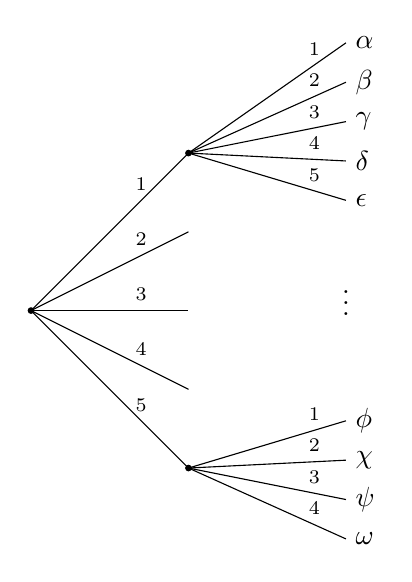
\begin{tikzpicture}[scale=2]
            \filldraw (0, 0) circle (0.5pt);
            \filldraw (1, 1) circle (0.5pt);
            \filldraw (1,-1) circle (0.5pt);
            \foreach \x in {1,...,5}{
                \pgfmathsetmacro\a{(3-\x)/2.0}
                \pgfmathsetmacro\b{(3-\x)/4.0 + 1.2}
                \draw (0, 0) --(1, \a) node[pos=0.7, above] {$\scriptstyle \x$};
                \draw (1, 1) -- (2, \b) node[pos=0.8, above] {$\scriptstyle \x$};
            };
            \foreach \x in {1,...,4}{
                \pgfmathsetmacro\c{(3-\x)/4.0 - 1.2}
                \draw (1, -1) -- (2, \c) node[pos=0.8, above] {$\scriptstyle \x$};
            };
            \node at (2, 0.1) {$\vdots$};
            \node [right] at (2, 1.7) {$\alpha$};
            \node [right] at (2, 1.45) {$\beta$};
            \node [right] at (2, 1.2) {$\gamma$};
            \node [right] at (2, 0.95) {$\delta$};
            \node [right] at (2, 0.7) {$\epsilon$};

            \node [right] at (2, -0.7) {$\phi$};
            \node [right] at (2, -0.95) {$\chi$};
            \node [right] at (2, -1.2) {$\psi$};
            \node [right] at (2, -1.45) {$\omega$};
        \end{tikzpicture}
    \end{center}
    Assuming $f$ is \hyperlink{def:prefixFreeCode}{prefix-free}, no codeword is the ancestor of any other. Now view the tree as a network with water being pumped in at a constant rate and dividing the flow equally at each node.

    The total amount of water we can extract at the codewords is $\sum_{i=1}^m a^{-s_i}$, which is therefore $\leq 1$.

    $(\Leftarrow)$ Conversely, suppose we can construct a prefix-free code with word lengths $s_1, \dotsc, s_m$, wlog $s_1 \leq s_2 \leq \dotsb \leq s_m$.
    We pick codewords of lengths $s_1, s_2, \dotsc$ sequentially ensuring previous codewords are not prefixes.
    Suppose there is no valid choice for the $r$th codeword.
    Then reconstructing the tree as above gives $ \sum_{i=1}^{r-1} a^{-s_i} = 1 $, contradicting our assumption.
    So we can construct a prefix-free code. (There is a more algebraic proof in Welsh.)
\end{proof}

\begin{nthm}[McMillan]\label{thm:mcmillan}
    Every \hyperlink{def:decipherable}{decipherable} \hyperlink{def:code}{code} satisfies \nameref{thm:kraft}.
\end{nthm}

\begin{proof}(Karush)
    Let $f: \Sigma_1 \to \Sigma_2^*$ be a \hyperlink{def:decipherable}{decipherable} \hyperlink{def:code}{code} with word lengths $s_1, \dotsc, s_m$, let $s = \max_{1 \leq i \leq m} s_i$.
    Let $r \in \N$,
    \begin{equation*}
        \left(\sum_{i=1}^m a^{-s_i}\right)^r = \sum_{l=1}^{rs} b_l a^{-l}
    \end{equation*}
    where $b_l$ is the \# of ways of choosing $r$ codewords of total length $l$. $f$ decipherable $\implies b_l \leq \abs{\Sigma_2}^l = a^l$.

    Thus \begin{gather*}\left(\sum_{i=1}^m a^{-s_i}\right)^r \leq \sum_{l=1}^{rs} a^l a^{-l} = rs \\
    \implies \sum_{i=1}^m a^{-s_i} \leq (rs)^{\frac{1}{r}} \to 1 \text{ as } r \to \infty.
    \end{gather*}
    (As $\frac{\log r + \log s}{r} \to 0$ as $r \to \infty$).
    \begin{equation*}
        \therefore \sum_{i=1}^m a^{-s_i} \leq 1.
    \end{equation*}
\end{proof}

\begin{cor}
    A decipherable code with prescribed word lengths exists iff there exists a prefix-free code with the same word lengths.
\end{cor}
So we can restrict our attention to prefix-free codes.

\subsection{Mathematical Entropy}
\begin{defi}[Entropy]\hypertarget{def:entropy}
    The entropy of $X$:
    \begin{equation*}
        H(X) = H(p_1, \dotsc, p_n) = -\sum_{i=1}^n p_i \log p_i
    \end{equation*}
    where, in this course, $\log = \log_2$.
\end{defi}

\begin{remark}
    \leavevmode
    \begin{enumerate}[label=(\roman*)]
        \item If $p_i = 0$, we take $p_i \log p_i=0$.
        \item $H(x) \geq 0$.
    \end{enumerate}
\end{remark}

\begin{eg}
    \leavevmode
    \begin{enumerate}[label=\arabic*.]
        \item Suppose $p_1 = p_2 = p_3 = p_4 = \frac{1}{4}$. We identify $\{x_1, x_2, x_3, x_4\}$ with \{HT, HT, TH, TT\}. Then $H(X) = 2$.
        \item Take $(p_1, p_2, p_3, p_4) = (\frac{1}{2}, \frac{1}{4}, \frac{1}{8}, \frac{1}{8})$.
            \begin{center}
                \begin{tikzpicture}[xscale=1.3, yscale=0.8]
                    \draw (0,0) -- (1,1);
                    \draw (0,0) -- (1, -1);
                    \draw (1, -1) -- (2, 0);
                    \draw (1, -1) -- (2, -2);
                    \draw (2, -2) -- (3, -1);
                    \draw (2, -2) -- (3, -3);
                    \node [right] at (1, 1) {$\frac{1}{2}$};
                    \node [right] at (2, 0) {$\frac{1}{4}$};
                    \node [right] at (3, -1) {$\frac{1}{8}$};
                    \node [right] at (3, -3) {$\frac{1}{8}$};
                \end{tikzpicture}
            \end{center}
            \begin{equation*}
                H(X) = \frac{1}{2} \times 1 + \frac{1}{4} \times 2 + \frac{1}{8} \times 3 + \frac{1}{8} \times 3 = \frac{7}{4}.
            \end{equation*}
            So example 1 is more random than example 2.
    \end{enumerate}
\end{eg}

\hyperlink{def:entropy}{Entropy} is a measure of `randomness' or `uncertainty'.
Consider a random variable $X$ taking values $x_1, \dotsc, x_n$ with probability $p_1, \dotsc, p_n$ ($\sum p_i = 1, 0 \leq p_i \leq 1$).
The entropy $H(X)$ is roughly speaking the expected number of tosses of a fair coin needed to simulate $X$ (or the expected number of yes/no questions we need to ask in order to establish the value of $X$).

% Lecture 3
\begin{eg}
    We toss a biased coin, $\Prob(\text{heads}) = p, \Prob(\text{tails}) = 1-p$. Write $H(p) = H(p, 1-p) = -p \log p - (1-p) \log (1-p)$.
    If $p=0$ or $1$, the outcome is certain and so $H(p)=0$. \hyperlink{def:entropy}{Entropy} is maximal where $p=\frac{1}{2}$, i.e. a fair coin.

    \begin{center}
        \begin{tikzpicture}
            \begin{axis}[ axis lines=center, xmin=-0.2, xmax=1.2, ymin=-0.2, ymax=1.2]
            \addplot [domain=0:1, samples=201]
            {-x*log2(x) - (1-x)*log2(1-x)};
            \end{axis}
        \end{tikzpicture}
    \end{center}
\end{eg}

Note the \hyperlink{def:entropy}{entropy} can also be viewed as the expected value of the information of $X$, where information is given by $I(X=x) = -\log_2 \Prob(X=x)$.
For example, if a coin always lands heads we gain no information from tossing the coin.
The entropy is the average amount of information conveyed by a random variable $X$.

\begin{nlemma}[Gibbs' Inequality]\label{lem:gibbs}
    Let $p_1, \dotsc, p_n$ and $q_1, \dotsc, q_n$ be probability distributions. Then
    \begin{equation*}
        -\sum p_i \log p_i \leq -\sum p_i \log q_i
    \end{equation*}
    with equality iff $p_i = q_i$.
\end{nlemma}
\begin{proof}
    Since $\log x = \frac{\ln x}{\ln 2}$ it suffices to prove the inequality with $\log$ replaced with $\ln$.
    Note $\ln x \leq x - 1$, equality iff $x=1$.
    \begin{center}
        \begin{tikzpicture}
            \begin{axis}[axis lines=center, axis equal, xmin=-1, xmax=6]
            \addplot [domain=0:8, samples=201]
            {ln(x)};
            \addplot [domain=-3:8, samples=21]
            {x-1};
            \end{axis}
        \end{tikzpicture}
    \end{center}
    Let $I = \set{1 \leq i \leq n | p_i \neq 0}$
    \begin{align*}
        \ln \frac{q_i}{p_i} &\leq \frac{q_i}{p_i} - 1 \quad \forall i \in I \\
        \sum_{i \in I} p_i \ln \frac{q_i}{p_i} &\leq \sum q_i - \underbrace{\sum p_i}_{=1} \leq 0 \\
        \implies -\sum_{i \in I} p_i \ln p_i &\leq -\sum_{i \in I} p_i \ln q_i \\
        \implies -\sum_{i =1}^n p_i \ln p_i &\leq -\sum_{i =1}^n p_i \ln q_i \\
    \end{align*}
    If equality holds then $\frac{q_i}{p_i} = 1$ $\forall i \in I$. So, $\sum_{i \in I} q_i = 1$ and hence $p_i = q_i$ for $1 \leq i \leq n$.
\end{proof}

\begin{cor}
    $H(p_1, \dotsc, p_n) \leq \log n$ with equality iff $p_1 = p_2 = \dotsb = p_n = \frac{1}{n}$.
\end{cor}
\begin{proof}
    Take $q_1 = q_2 = \dotsc = q_n = \frac{1}{n}$ in \nameref{lem:gibbs}.
\end{proof}

Suppose we have two alphabets $\Sigma_1, \Sigma_2$ with $\abs{\Sigma_1} = m$ and $\abs{\Sigma_2} = a$, for $m \geq 2$ and $a \geq 2$.
We model the source as a sequence of random variables $X_1, X_2, \dotsc$ taking values in $\Sigma_1$.
\begin{defi}[Memoryless source]\hypertarget{def:memoryless}
    A \textbf{Bernoulli} or \textbf{memoryless} source is a sequence of independently, identically distributed random variables.
\end{defi}
That is, for each $\mu \in \Sigma_1$, $\Prob(X_i = \mu)$ is independent of $i$ and independent of all past and future symbols emitted. Thus
\begin{equation*}
    \Prob(X_1= x_1, X_2 = x_2, \dotsc, X_k = x_k) = \prod_{i = 1}^k \Prob(X_i = x_i).
\end{equation*}
Let $\Sigma_1 = \{\mu_1, \dotsc, \mu_n\}$, $p_i = \Prob(X=\mu_i)$ (assume $p_i > 0$).
\begin{defi}[Expected word length]\hypertarget{def:ewl}
    The \textbf{expected word length} of a code $f: \Sigma_1 \to \Sigma_2^*$ with word lengths $s_1, \dotsc, s_m$ is $E(S) = \sum_{i=1}^m p_i s_i$.
\end{defi}

\begin{defi}[Optimal code]\hypertarget{def:optCode}
    A \hyperlink{def:code}{code} $f:\Sigma_1 \to \Sigma_2^*$ is \textbf{optimal} if it has the shortest possible \hyperlink{def:ewl}{expected word length} among \hyperlink{def:decipherable}{decipherable} codes.
\end{defi}
\begin{nthm}[Shannon's Noiseless Coding Theorem]\label{thm:noiselessCode}
    The minimum \hyperlink{def:ewl}{expected word length} of a \hyperlink{def:decipherable}{decipherable code} $f: \Sigma_1 \to \Sigma_2^*$ satisfies
    \begin{equation*}
        \frac{H(X)}{\log a} \leq E(S) < \frac{H(X)}{\log a} + 1
    \end{equation*}
\end{nthm}
\begin{proof}
    The lower bound is given by combining \nameref{lem:gibbs} and \nameref{thm:kraft}.
    Let $q_i = \frac{a^{-s_i}}{c}$ where $c = \sum a^{-s_i} \leq 1$ by \nameref*{thm:kraft}.
    Note $\sum q_i = 1$.
    \begin{align*}
        H(X) = -\sum p_i \log p_i &\leq -\sum_i p_i \log q_i \\
                                  &= \sum p_i (s_i \log a + \log c) \\
                                  &= \left(\sum p_i s_i\right) \log a + \underbrace{\log c}_{\leq 0} \leq E(S) \log a\\
        \implies \frac{H(X)}{\log a} &\leq E(S)
    \end{align*}
    We get equality $\iff p_i = a^{-s_i}$ for some integers $s_i$.
    For the upper bound put
    \begin{equation*}
        s_i = \ceil{-\log_a p_i}
    \end{equation*}
    where $\ceil{x}$ means least integer $\geq x$.

    We have
    \begin{gather*}
        - \log_a p_i \leq s_i < - \log_a p_i + 1 \\
        \implies a^{-s_i} \leq p_i \implies \sum a^{-s_i} \leq \sum p_i \leq 1.
    \end{gather*}
    So by \cref{thm:kraft}, $\exists$ a prefix-free code with word lengths $s_1, \dotsc, s_m$.
    Also,
    \begin{align*}
        E(S) &= \sum p_i s_i \\
             &< p_i (- \log_a p_i + 1) \\
             &= \frac{H(X)}{\log a} + 1 \qedhere
    \end{align*}
\end{proof}
\begin{remark}
    The lower bound holds for all \hyperlink{def:decipherable}{decipherable} \hyperlink{def:code}{codes}.
\end{remark}

\subsection{Shannon-Fano coding}
Follows from above proof.
\hypertarget{def:shannonFanoCode}Set $s_i = \ceil{-\log_a p_i}$ and construct a \hyperlink{def:prefixFreeCode}{prefix-free code} with word lengths $s_1, \dotsc, s_m$ by taking the $s_i$ in increasing order ensuring that previous \hyperlink{def:code}{codewords} are not prefixes.
\nameref{thm:kraft} ensures there is enough room.
\begin{eg}
    Suppose $\mu_1, \dotsc, \mu_5$ are emitted with probabilities $0.4, 0.2, 0.2, 0.1, 0.1$.

    A \hypertarget{ex:shannonfano1}{possible \hyperlink{def:shannonFanoCode}{Shannon-Fano}} code (with $a=2$, $\Sigma_2 = \{0, 1\}$) has
    \begin{center}
    \begin{tabular}{c c c}
        $p_i$ & $\ceil{-\log_2 p_i}$ & \\
        \hline
        0.4 & 2 & 00 \\
        0.2 & 3 & 010 \\
        0.2 & 3 & 100 \\
        0.1 & 4 & 1100 \\
        0.1 & 4 & 1110
    \end{tabular}
    \end{center}
    This has \hyperlink{def:ewl}{expected word length}
    \begin{align*}
        &= 2 \times 0.4 + 3 \times 0.2 + 3 \times 0.2 + 4 \times 0.1 + 4 \times 0.1 \\
        &= 2.8.
    \end{align*}
    compare $H(X) \approx 2.12$.
\end{eg}

\subsection{Huffman coding}
For simplicity, take $a=2$.
Take $\Sigma_1=\{\mu_1, \dotsc, \mu_m\}$ with $p_i = \Prob(X = \mu_i)$. Without loss of generality, $p_1 \geq p_2 \geq \dotsb \geq p_m$.
\hypertarget{def:huffmanCode}Huffman coding is defined inductively.

If $m=2$, assign codewords $0$ and $1$. If $\mu > 2$, find a Huffman coding in the case of messages $\mu_1, \mu_2, \dotsc, \nu$, with probabilities $p_1, p_2, \dotsc, p_{m-1} + p_m$.

Append $0$ (resp, $1$) to the codeword for $\nu$ to give a codeword for $\mu_{m-1}$ (resp, $\mu_m$).

\begin{remark}
    \leavevmode
    \begin{enumerate}[label=\roman*)]
        \item This construction gives a \hyperlink{def:prefixFreeCode}{prefix-free} code.
        \item We exercise some choice when some of the $p_i$ are equal. So \hyperlink{def:huffmanCode}{Huffman codes} are not unique.
    \end{enumerate}
\end{remark}

\begin{eg}
    Use the same \hyperlink{ex:shannonfano1}{example probabilities} as earlier.
    \begin{equation*}
        \begin{tikzcd}[column sep=large, arrows={start anchor=east, end anchor=west, dash}]
                0.4 \quad \color{bblue}(1)
              & 0.4 \quad \color{bblue}(1)
              & 0.4 \quad \color{bblue}(1)
              & 0.6 \quad \color{bblue}({\color{bred}0}) \\
                0.2 \quad \color{bblue}(00)
              & 0.2 \quad \color{bblue}(00)
              & 0.4 \quad \color{bblue}(0{\color{bred}1}) \ar[ur]
              & 0.4 \quad \color{bblue}(1) \\
                0.2 \quad \color{bblue}(011)
              & 0.2 \quad \color{bblue}(01{\color{bred}1}) \ar[ur]
              & 0.2 \quad \color{bblue}(0{\color{bred}0}) \ar[uur] \\
                0.1 \quad \color{bblue}(010{\color{bred}1}) \ar[r]
              & 0.2 \quad \color{bblue}(01{\color{bred}0}) \ar[uur] \\
                0.1 \quad \color{bblue}(010{\color{bred}0}) \ar[ur]
    \end{tikzcd}
    \end{equation*}
    So $\{1, 00, 011, 0101, 0100\}$ is the \hyperlink{def:prefixFreeCode}{prefix-free code} constructed. The \hyperlink{def:ewl}{expected word length} is:
    \begin{align*}
        &= 1 \times 0.4 + 2 \times 0.2 + 2 \times 0.2 + 4 \times 0.1 + 4 \times 0.1 \\
        &= 0.4 + 0.4 + 0.6 + 0.4 + 0.4\\
        &= 2.2.
    \end{align*}
    This is better than \hyperlink{def:shannonFanoCode}{Shannon-Fano}, which gave 2.8.
\end{eg}

\begin{nthm}\label{thm:huffOpt}
    \hyperlink{def:huffmanCode}{Huffman coding} is \hyperlink{def:optCode}{optimal}.
\end{nthm}
\begin{nlemma}\label{lem:1.6}
    Suppose we have $\mu_1, \dotsc, \mu_m \in \Sigma_1$ emitted with probabilities $p_1, \dotsc, p_m$.
    Let $f$ be an \hyperlink{def:optCode}{optimal} \hyperlink{def:prefixFreeCode}{prefix-free} \hyperlink{def:code}{code}, with word lengths $s_1, \dotsc, s_m$.
    Then
    \begin{enumerate}[label=\roman*)]
        \item If $p_i > p_j$, then $s_i \leq s_j$.
        \item $\exists$ two \hyperlink{def:code}{codewords} of maximal length which are equal up to the last digit.
    \end{enumerate}
\end{nlemma}

\begin{proof}
    \leavevmode
    \begin{enumerate}[label=\roman*)]
        \item If not, then swap the $i$th and $j$th \hyperlink{def:codewords}{codewords}.
            This decreases the \hyperlink{def:ewl}{expected word length}, contradicting $f$ \hyperlink{def:optCode}{optimal}.
        \item If not, then either only one codeword of maximal length, or any two codewords of maximal length differ before the last digit.
            In either case, delete the last digit of each codeword of maximal length.
            This maintains the \hyperlink{def:prefixFreeCode}{prefix-free} condition, contradicting $f$ optimal. \qedhere
    \end{enumerate}
\end{proof}
\begin{proof}[Proof of \cref{thm:huffOpt}]
    We only take the case $a=2$.
    We show by induction on $m$ that any \hyperlink{def:huffmanCode}{Huffman code} of size $m$ is \hyperlink{def:optCode}{optimal}. \\
    For $m=2$, \hyperlink{def:code}{codewords} $0,1$ are optimal. \\
    For $m>2$, say source $X_m$ emits $\mu_1, \dotsc, \mu_m$ with probabilities $p_1 \geq p_2 \geq \dotsc \geq p_m$ while source $X_{m-1}$ emits $\mu_1, \dotsc, \mu_{m-2}, \nu$ with probabilities $p_1, \dotsc, p_{m-2}, p_{m-1} + p_m$.

    We construct a Huffman coding $f_{m-1}$ for $X_{m-1}$ and extend to a Huffman coding for $X_m$.
    Then the \hyperlink{def:ewl}{expected codeword length} satisfies:
    \begin{equation*}
        E(s_m) = E(s_{m-1}) + p_{m-1} + p_m \label{eq:4dag} \tag{$\dagger$}
    \end{equation*}
    Let $f_m'$ be an optimal code for $X_m$, WLOG $f_m'$ prefix-free.
    \Cref{lem:1.6} tells us that by shuffling codewords, we may assume that the last two codewords are of maximal length and differ only in the last digit, say $y_0$ and $y_1$ for some string $y$.

    We define a code $f_{m-1}'$ for $X_{m-1}$ with
    \begin{align*}
        f_{m-1}'(\mu_i) &= f'_m(\mu_i) \quad \forall 1 \leq i \leq m-2 \\
        f'_{m-1}(\nu) &= y.
    \end{align*}
    Then $f'_{m-1}$ is a prefix-free code, and the expected word length satisfies
    \begin{equation*}
        E(s'_m) = E(s'_{m-1}) + p_{m-1} + p_m \tag{$\ddagger$} \label{eq:4ddag}
    \end{equation*}
    Induction hypothesis tells us $f_{m-1}$ is optimal, so $E(s_{m-1}) \leq E(s'_{m-1})$. Hence $E(s_m) \leq E(s'_m)$ by \eqref{eq:4dag}, \eqref{eq:4ddag}.
    So $f_m$ optimal.
\end{proof}
\begin{remark}
    Not all \hyperlink{def:optCode}{optimal} codes are \hyperlink{def:huffmanCode}{Huffman}. For instance, take $m=4$, and probabilities $0.3, 0.3, 0.2, 0.2$. An optimal code is given by $00, 01, 10, 11$, but this is not Huffman.

    But, the previous result says that if we have a prefix-free optimal code with word lengths $s_1, \dotsc, s_m$ and associated probabilites $p_1, \dotsc, p_m$, $\exists$ a Huffman code with these word lengths.
\end{remark}

\begin{defi}[Joint entropy]\hypertarget{def:jointEntropy}
    The \textbf{joint entropy} of $X$ and $Y$ is
    \begin{equation*}
        H(X,Y) = - \sum_{x \in \Sigma_1} \sum_{y \in \Sigma_2} \Prob(X=x, Y=y) \log \Prob(X=x, Y=y).
    \end{equation*}
\end{defi}

\begin{nlemma}
    $\hyperlink{def:jointEntropy}{H(X, Y)} \leq \hyperlink{def:entropy}{H}(X) + H(Y)$, with equality $\iff X,Y$ independent.
\end{nlemma}

\begin{proof}
    Take $\Sigma_1 = \{x_1, \dotsc, x_m\}$, $\Sigma_2 = \{y_1, \dotsc, y_n\}$. Let $p_{ij} = \Prob(X=x_i, Y=y_j)$, as well as $p_i = \Prob(X=x_i)$, $q_i = \Prob(Y=y_i)$.
    Apply \nameref{lem:gibbs} to the distributions $p_{ij}$ and $p_i q_j$:
    \begin{align*}
        -\sum p_{ij} \log(p_{ij}) &\leq -\sum p_{ij} \log(p_i q_j) \\
                                  &= - \sum_i \left(\sum_j p_{ij} \log p_i\right) - \sum_j \left(\sum_i p_{ij} \log q_j\right) \\
                                  &= -\sum p_i \log p_i - \sum q_j \log q_j
    \end{align*}
    That is, $H(X,Y) \leq H(X) + H(Y)$.
    Equality $\iff p_{ij} = p_i q_j \forall i, j \iff X, Y$ independent.
\end{proof}

% Lecture 5
Suppose a source $\Omega$ produces a stream $X_1, X_2, \dotsc$ of random variables with values in $\Sigma$.
The probability mass function (p.m.f.) of $X^{(n)} = (X_1, \dotsc, X_n)$ is given by
\begin{equation*}p_n(x_1, \dotsc, x_n) = \Prob(X_1, \dotsc, X_n = x_1, \dotsc, x_n) \quad \forall x_1, \dotsc, x_n \in \Sigma^n\end{equation*}
Now,
\begin{align*}
    p_n &: \Sigma^n \to \R \\
    X^{(n)} &: \Omega \to \Sigma^n\\
    \shortintertext{can form}
    p_n(X^{(n)})&: \Sigma \xrightarrow{X^{(n)}} \Sigma^n \xrightarrow{p_n} \R
\end{align*}
a random variable sending $\omega \mapsto p_n(X^{(n)} = X^{(n)} (\omega))$.
\begin{eg}
    Take $\Sigma = \{A, B, C\}$, with
    \begin{equation*}
        X^{(2)} =
        \begin{cases}
            AB & p=0.3 \\
            AC & p=0.1 \\
            BC & p=0.1 \\
            BA & p=0.2 \\
            CA & p=0.25 \\
            CB & p=0.05 \\
        \end{cases}
    \end{equation*}
    So, $p_2(AB) = 0.3$, etc, and $p_2(X^{(2)})$ takes values
    \begin{equation*}
        p_2(X^{(2)}) =
        \begin{cases}
            0.3 & p=0.3 \\
            0.1 & p=0.2 \\
            0.2 & p=0.2 \\
            0.25 & p=0.25 \\
            0.05 & p=0.05 \\
        \end{cases}
    \end{equation*}
\end{eg}

\begin{defi}[Convergence in probability]\hypertarget{def:probConverge}
    A sequence of random variables $X_1, X_2, \dotsc$ \textbf{converges in probability} to $c \in \R$, written $X_n \xlongrightarrow{p} c$ as $n \to \infty$, if
    \begin{equation*}
        \forall \epsilon > 0 \quad \Prob(\abs{X_n - c} \leq \epsilon) \to 1 \quad \text{as } n \to \infty.
    \end{equation*}
    So, $X_n$ and $c$ can take very different values for large $n$, but only on a set with small probability.
\end{defi}

\begin{thm}[Weak law of large numbers]\hypertarget{def:wlln}
    $X_1, X_2, \dotsc$ an independent, identically distributed sequence of random variables with finite expected value $\mu$, then
    \begin{equation*}
        \frac{1}{n} \sum_{i=1}^n X_i \probConv \mu \quad \text{as } n \to \infty.
    \end{equation*}
\end{thm}
\begin{eg}[Application]
    Take $X_1, X_2, \dotsc$ a \hyperlink{def:memoryless}{Bernoulli source}. Then $p(X_1), p(X_2), \dotsc$ are i.i.d. random variables
    \begin{align*}
        p(X_1, \dotsc, X_n) &= p(X_1) \dotsc p(X_n) \\
        -\frac{1}{n} \log p(X_1, \dotsc, X_n) &= -\frac{1}{n} \sum_{i=1}^n \log p(X_i) \probConv E(-\log p(X_1)) = H(X_1) \quad \text{as } n \to \infty.
    \end{align*}
\end{eg}
\begin{defi}[Asymptotic Equipartition Property]
    \leavevmode

    A source $X_1, X_2, \dotsc$ satisfies the \hypertarget{def:aep}{\textbf{Asymptotic Equipartition Property}} (AEP) if for some $H\geq 0$ we have
    \begin{equation*}
        -\frac{1}{n} \log p(X_1, \dotsc, X_n) \xrightarrow{p} H \quad \text{as } n \to \infty.
    \end{equation*}
\end{defi}
\begin{eg}
    Consider a coin, $p(H) = p$. If coin tossed $N$ times, expect approximately $pN$ heads and $(1-p)N$ tails.
    \begin{align*}
        &\Prob(\text{particular sequence of $pN$ heads and $(1-p)N$ tails}) \\
        =&p^{pN} (1-p)^{(1-p)N}\\
        =&2^{N(p \log p) + (1-p) \log (1-p)} = 2^{-N H(A)}
    \end{align*}
    where $A$ is the result of an independent coin toss.
    So, with high probability we will get a typical sequence, and its probability will be close to $2^{-NH(A)}$.
\end{eg}
\begin{nlemma}
    A source $X_1, \dotsc, X_n$ satisfies \hyperlink{def:aep}{AEP} iff it satisfies the following.
    \begin{gather*}
        \forall \epsilon > 0, \, \exists n_0(\epsilon) \text{ such that } \forall n \geq n_0(\epsilon) \, \exists \text{ a `\hypertarget{def:typicalSet}{typical set}' } T_n \subset \Sigma^n \text{ with}
    \end{gather*}
    \begin{equation*}
        \begin{gathered}
        \Prob((X_1, \dotsc, X_n) \in T_n) > 1 - \epsilon \\
        2^{-n(H+\epsilon)} \leq p(x_1, \dotsc, x_n) \leq 2^{-n(H-\epsilon)}\quad \forall (x_1, \dotsc, x_n) \in T^n
        \end{gathered}
        \tag{$*$} \label{eq:5star}
    \end{equation*}
\end{nlemma}
\begin{proof}[Sketch proof]
    \hyperlink{def:aep}{AEP} $\Rightarrow$ \eqref{eq:5star}.
    Take
    \begin{align*}
        T_n &= \Set{(x_1, \dotsc, x_n) \in \Sigma^n | \abs{-\frac{1}{n} \log p(x_1, \dotsc, x_n) - H} < \epsilon} \\
            &= \Set{(x_1, \dotsc, x_n) \in \Sigma^n | 2^{-n(H+\epsilon)} \leq p(x_1, \dotsc, x_n) \leq 2^{-n(H-\epsilon)}} \\
    \end{align*}
    \eqref{eq:5star} $\Rightarrow$ \hyperlink{def:aep}{AEP}
    \begin{equation*}
        \Prob\left(\abs{- \frac{1}{n} p(X_1, \dotsc, X_n) - H} < \epsilon\right) \geq \Prob(T_n) \to 1 \quad \text{as } n \to \infty. \qedhere
    \end{equation*}
\end{proof}
\begin{defi}[Reliably encodable]\hypertarget{def:reliablyEncode}
    A source $X_1, X_2, \dotsc$ is \textbf{reliably encodable} at rate $r$ if $\exists A_n \subset \Sigma^n$ for each $n$ such that
    \begin{enumerate}[label=(\roman*)]
        \item $\frac{\log \abs{A_n}}{n} \to r \quad \text{as } n \to \infty$
        \item $\Prob((X_1, \dotsc, X_n) \in A_n) \to 1 \quad \text{as } n \to \infty$.
    \end{enumerate}
    So, in principle you can encode at rate almost $r$ with negligible error for long enough strings.
\end{defi}
So, if $\abs{\Sigma}=a$, you can \hyperlink{def:reliablyEncode}{reliably encode} at rate $\log a$. However you can often do better.
For example, consider telegraph English with 26 letters and a space. $27 \approx 2^{4.756}$, so can encode at rate of $4.76$ bits/letter. But much lower rates suffice, as there is a lot of redundancy in the English language.
Hence the following definition.
\begin{defi}[Information rate]\hypertarget{def:informationRate}
    The \textbf{information rate} $H$ of a source is the infimum of all values at which it is \hyperlink{def:reliablyEncode}{reliably encodable}.
\end{defi}
Roughly, $nH$ is the number of bits required to encode $(X_1, \dotsc, X_n)$.
\begin{nthm}[Shannon's first coding theorem]
    If a source satisfies \hyperlink{def:aep}{AEP} with some constant $H$, then the source has information rate $H$.
\end{nthm}
\begin{proof}Let $\epsilon > 0$ and let $T_n \subset \Sigma^n$ be \hyperlink{def:typicalSet}{typical sets}.
    Then for sufficiently large $n \geq n_0(\epsilon)$,
    \begin{equation*}
        p(x_1, \dotsc, x_n) \geq 2^{-n (H + \epsilon))} \quad \forall (x_1, \dotsc, x_n) \in T^n.
    \end{equation*}
    So,
    \begin{gather*}
        \Prob(\left(X_1, \dotsc, X_n\right) \in T_n) \geq 2^{-n(H+\epsilon)} \abs{T_n} \\
        \implies \abs{T_n} \leq 2^{n(H+\epsilon)}
    \end{gather*}
    therefore the source is \hyperlink{def:reliablyEncode}{reliably encodable} at rate $H+\epsilon$.

    Conversely, if $H=0$, done. Otherwise, pick $0 < \epsilon < \frac{H}{2}$. Suppose the source is reliably encodable at rate $H - 2 \epsilon$, say with sets $A_n$.
    \begin{gather*}
        p(x_1, \dotsc, x_n) \leq 2^{-n(H-\epsilon)} \quad \forall (x_1, \dotsc, x_n) \in T_n \\
        \begin{aligned}
            \implies \Prob((x_1, \dotsc, x_n) \in A_n \cap T_n) &\leq 2^{-n (H-\epsilon)} \abs{A_n} \\
            \implies \frac{\log \Prob(A_n \cap T_n)}{n} &\leq -(H-\epsilon) + \frac{\log \abs{A_n}}{n} \\
                                                    &\to -(H-\epsilon) + (H-2 \epsilon) = -\epsilon \quad \text{as } n \to \infty. \qedhere
        \end{aligned}
    \end{gather*}
    % A few things missing here - make sure to fill in!
\end{proof}

% lecture 6
\clearpage
\section{Error Control Codes}
\begin{defi}[Binary code]\hypertarget{def:binaryCode}
    A $[n, m]$ \textbf{binary code} is a subset $C \subset \{0, 1\}^n$ of size $\abs{C}=m$. We say $C$ has length $n$.
    The elements of $C$ are called \textbf{codewords}.
\end{defi}
We use a $[n, m]$-code to send one of $m$ possible messages through a \hyperlink{def:bsc}{BSC} making use of the channel $n$ times.
\begin{center}
    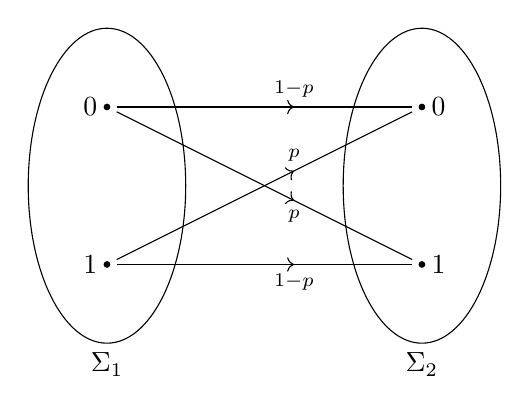
\begin{tikzpicture}
        \draw (-2, 0) circle [x radius=1cm, y radius=2cm] node [below=2cm] {$\Sigma_1$};
        \draw ( 2, 0) circle [x radius=1cm, y radius=2cm] node [below=2cm] {$\Sigma_2$};

        \node (0l) at (-2, 1) {};
        \node (1l) at (-2,-1) {};

        \node (0r) at (2, 1) {};
        \node (1r) at (2,-1) {};

        \filldraw (0l) circle (1pt) node [left] {0};
        \filldraw (1l) circle (1pt) node [left] {1};
        \filldraw (0r) circle (1pt) node [right] {0};
        \filldraw (1r) circle (1pt) node [right] {1};

        \begin{scope}[decoration={
            markings,
            mark=at position 0.6 with {\arrow{>}}}
            ]
            \draw[postaction={decorate}] (0l) -- (0r)
                node [above,align=center,pos=0.6] {$\scriptstyle 1-p$};
            \draw[postaction={decorate}] (0l) -- (1r)
                node [below,align=center,pos=0.6] {$\scriptstyle p$};
            \draw[postaction={decorate}] (1l) -- (0r)
                node [above,align=center,pos=0.6] {$\scriptstyle p$};
            \draw[postaction={decorate}] (1l) -- (1r)
                node [below,align=center,pos=0.6] {$\scriptstyle 1-p$};
        \end{scope}
    \end{tikzpicture}
\end{center}
\begin{defi}[Information rate]\hypertarget{def:infoRate}
    The \textbf{information rate} of $C$ is
    \begin{equation*}
        \rho(C) = \frac{\log{m}}{n}
    \end{equation*}
    where we continue to use $\log = \log_2$.
\end{defi}

Note since $C\subset\{0, 1\}^n$, $\rho(C) \leq 1$, with equality iff $C = \{0, 1\}^n$.
A \hyperlink{def:binaryCode}{code} with size $m=1$ has \hyperlink{def:infoRate}{information rate} 0.

We aim to design codes with both a large information rate and a small error rate, which are contradicting aims.
The error rate depends on the decoding rule. We consider 3 possible rules.
\begin{enumerate}[label=(\roman*)]\hypertarget{def:idealObserver}
    \item The \textbf{ideal observer} decoding rule decodes $x \in \{0, 1\}^n$ as the \hyperlink{def:binaryCode}{codeword} $c$ maximising $\Prob(c\text{ sent} \mid x\text{ received})$.
    \item \hypertarget{def:maximumLikelihood}{The} \textbf{maximum likelihood} decoding rule decodes $x \in \{0, 1\}^n$ as the codeword $c$ maximising $\Prob(x\text{ received} \mid c\text{ sent})$.
    \item \hypertarget{def:minimumDistanceRule}{The} \textbf{minimum distance} decoding rule decodes $x \in \{0, 1\}^n$ as the codeword $c$ minimising $\#\set{1 \leq i \leq n | x_i \neq c_i}$.
\end{enumerate}
\begin{remark}
    Some convention should be agreed in the case of a `tie', e.g.\ choose at random, or ask for message to be sent again.
\end{remark}
\begin{nlemma}\label{lem:2.1}
    If all messages are equally likely, then the \hyperlink{def:idealObserver}{ideal observer} and \hyperlink{def:maximumLikelihood}{maximum likelihood rule} agree.
\end{nlemma}
\begin{proof}
    By Bayes' rule,
    \begin{align*}
        \Prob(c \text{ sent} \mid x \text{ received}) &= \frac{\Prob(c \text{ sent}, x \text{ received})}{\Prob(x \text{ received})} \\
                                               &= \frac{\Prob(c \text{ sent})}{\Prob(x \text{ received})} \Prob(x \text{ received} \mid c \text{ sent}).
    \end{align*}
    We suppose $\Prob(c \text{ sent})$ is independent of $c$. So for fixed $x$, maximising $\Prob(c \text{ sent} \mid x \text{ received}) $ is the same as maximising $\Prob(x \text{ received} \mid c \text{ sent})$.
\end{proof}

\begin{defi}[Hamming distance]\label{def:hammingDistance}
    Let $x, y \in \{0, 1\}^n$. Then \textbf{Hamming distance} between $x$ and $y$ is
    \begin{equation*}d(x, y) = \# \set{1 \leq i \leq n | x_i \neq y_i}.\end{equation*}
\end{defi}
\begin{nlemma}\label{lem:2.2}
    If $p < \frac{1}{2}$, then \hyperlink{def:maximumLikelihood}{maximum likelihood} and \hyperlink{def:minimumDistanceRule}{minimum distance} agree.
\end{nlemma}
\begin{proof}
    Suppose $\hyperlink{def:hammingDistance}{d(x, c)} = r$,
    \begin{equation*}
        \Prob(x \text{ received} \mid c \text{ sent}) = p^r (1-p)^{n-r} = (1-p)^n \left(\frac{p}{1-p}\right)^r.
    \end{equation*}
    Since $p < \frac{1}{2}$, $\frac{p}{1-p} < 1$. So choosing $c$ to maximise $\Prob(x \text{ received} \mid c \text{ sent})$ is the same as choosing $c$ to minimise $d(x, c)$.
\end{proof}
Note we assumed $p < \frac{1}{2}$, which is not unreasonable.
\begin{eg}
    Suppose codewords $000$ and $111$ are sent with probabilities $\alpha = \frac{9}{10}$ and $1-\alpha = \frac{1}{10}$ respectively. We use a \hyperlink{def:bsc}{BSC} with $p = \frac{1}{4}$.
    If we receive $110$, how should it be decoded?
    Clearly \hyperlink{def:minimumDistanceRule}{minimum distance} and therefore \hyperlink{def:maximumLikelihood}{maximum likelihood} (by \cref{lem:2.2}) say decode as $111$.
    For \hyperlink{def:idealObserver}{ideal observer:}
    \begin{align*}
        \Prob(000 \text{ sent} \mid 110 \text{ received}) &= \frac{\Prob(000 \text{ sent} , 110 \text{ received})}{\Prob(110 \text{ received})} \\
                                                   &= \frac{\alpha p^2 (1-p)}{\alpha p^2 (1-p) + (1-\alpha) p (1-p)^2} \\
                                                   &= \frac{\alpha p}{\alpha p + (1-\alpha) (1-p)} \\
                                                   &= \frac{9/40}{9/40 + 3/40} = \frac{3}{4} \\
        \Prob(000 \text{ sent} \mid 110 \text{ received}) &= \frac{(1-\alpha) p^2 (1-p)}{(1-\alpha) p^2 (1-p) + \alpha p (1-p)^2} \\
                                                   &= \frac{(1-\alpha)(1-p)}{(1-\alpha)(1-p) + \alpha p} \\
                                                   &= \frac{3/40}{9/40 + 3/40} = \frac{1}{4}.
    \end{align*}
    So the ideal observer rule says decode as $000$.
\end{eg}
\begin{remark}
    The \hyperlink{def:idealObserver}{ideal observer} rule is also known as the minimum-error rule.
    But it does rely on knowing the probabilities of the codewords sent.
\end{remark}
From now on, we use \hyperlink{def:minimumDistanceRule}{minimum distance} decoding.
\begin{defi}
    For a \hyperlink{def:binaryCode}{binary code} $C$,
    \begin{enumerate}[label=(\roman*)]
        \item $C$ is \hypertarget{def:errorDet}{\textbf{$d$-error detecting}} if changing at most $d$ letters of a codeword cannot give another codeword.
        \item $C$ is \hypertarget{def:errorCor}{\textbf{$e$-error correcting}} if knowing that the string received has at most $e$ errors is sufficient to determine which codeword was sent.
    \end{enumerate}
\end{defi}
\begin{eg} \leavevmode
    \begin{enumerate}[label=\arabic*.]
        \item The \hypertarget{def:repetitionCode}{repetition code} of length $n$ has:
            \begin{equation*}
                C = \{\underbrace{0\dotsm0}_n, \underbrace{1 \dotsm1}_n\}
            \end{equation*}
            This is an \hyperlink{def:binaryCode}{$[n, 2]$-code}. It is $n-1$ \hyperlink{def:errorDet}{error detecting}, and $\floor{\frac{n-1}{2}}$ \hyperlink{def:errorCor}{error correcting}.
            But it has \hyperlink{def:infoRate}{information rate} $= \frac{1}{n}$.
        \item The \hypertarget{def:parityCheckCode}{simple parity check} code of length $n$ (also known as paper tape code).
            We view $\{0, 1\} = \mathbb{F}_2 = \Z/2\Z$ (i.e.\ do arithmetic modulo $2$).
            \begin{equation*}
                C = \Set{(x_1, \dotsc, x_n) \in \{0, 1\}^n | \sum_{i=1}^n x_i = 0}.
            \end{equation*}
            This is a \hyperlink{def:binaryCode}{$[n, 2^{n-1}]$-code}.
            It is $1$-\hyperlink{def:errorDet}{error detecting} and $0$-\hyperlink{def:errorCor}{error correcting}.
            It has \hyperlink{def:infoRate}{information rate} $\frac{n-1}{n}$.
        \item \hypertarget{def:hammingCode}{Hamming's original} code (1950). % this example was lecture 7
            Let $C \subseteq \mathbb{F}_2^7$ be defined by
            \begin{align*}
                c_1 + c_3 + c_5 + c_7 &= 0 \\
                c_2 + c_3 + c_6 + c_7 &= 0 \\
                c_4 + c_5 + c_6 + c_7 &= 0
            \end{align*}
            where all arithmetic is modulo 2.
            Since we may choose $c_3, c_5, c_6, c_7$ freely, the $c_1, c_2, c_4$ are uniquely determined.
            So we get $\abs{C} = 2^4$ i.e.\ $C$ is a $[7,16]$-\hyperlink{def:binaryCode}{code}.
            It has \hyperlink{def:infoRate}{information rate} $\frac{\log m} {n} = \frac{4}{7}$.
            Note $c_{3,5,6,7}$ are free, $c_{1,2,4}$ are check digits.

            Suppose we receive $x \in \mathbb{F}_2^7$. We form the syndrome $z_x = (z_1, z_2, z_4)$ where
            \begin{align*}
                z_1 &= x_1 + x_3 + x_5 + x_7 \\
                z_2 &= x_2 + x_3 + x_6 + x_7 \\
                z_4 &= x_4 + x_5 + x_6 + x_7.
            \end{align*}
            If $x \in C$, then $z = (0,0,0)$. If $\hyperlink{def:hammingDistance}{d}(x, c) = 1$ for some $c \in C$, then the place where $x$ and $c$ differ is given by $z_1 + 2 z_2 + 4z_4$ (not modulo 2).
            Since if $x = c+ e_i$ where $e_i = 0\dotso 010\dotso 0$ ($1$ in the $i$th place), then the syndrome of $x$ is the syndrome of $e_i$.
            For example the syndrome of $e_3$ is $(1, 1, 0)$, the binary expansion of $3$.
            True in fact for each $1 \leq i \leq 7$.
    \end{enumerate}
\end{eg}

\begin{remark}
    Suppose we change our \hyperlink{def:binaryCode}{code} $C \subset \{0, 1\}^n$ by using the same permutation to reorder each \hyperlink{def:binaryCode}{codeword}.
    This gives a code with the same mathematical properties (e.g.\ \hyperlink{def:infoRate}{information rate}, \hyperlink{def:errorDet}{error detection rate}).
    We say such codes are equivalent.
\end{remark}

% lecture 7

\begin{nlemma}\label{lem:2.3}
    The \hyperlink{def:hammingDistance}{Hamming distance} is a metric on $\mathbb{F}_2^n$.
\end{nlemma}

\begin{proof}
    Clearly $d(x, y) \geq 0$ with equality iff $x=y$.
    Also $d(x, y) = d(y, x)$. Check triangle inequality, let $x, y, z \in \mathbb{F}_2^n$:
    \begin{gather*}
        \set{1 \leq i \leq n | x_i \neq z_i} \subseteq
        \set{1 \leq i \leq n | x_i \neq y_i} \cup
        \set{1 \leq i \leq n | y_i \neq z_i} \\
        \implies d(x, z) \leq d(x, y) + d(y, z) \qedhere
    \end{gather*}
\end{proof}
\begin{remark}
    We could also write $d(x, y) = \sum_{i=1}^n d_1(x_i, y_i)$ where $d_1$ is the discrete metric on $\{0, 1\}$.
\end{remark}

\begin{defi}[Minimum distance]\label{def:minimumDistanceCode}
    The \textbf{minimum distance} of a code $C$ is the smallest \hyperlink{def:hammingDistance}{Hamming distance} between distinct codewords.
\end{defi}
\begin{notation}
    An \hyperlink{def:binaryCode}{$[n, m]$-code} with \hyperlink{def:minimumDistanceCode}{minimum distance} $d$ is sometimes called an \hypertarget{def:nmdCode}{$\bm{[n, m, d]}$\textbf{-code}}.
\end{notation}
\begin{remark}\leavevmode
    \begin{itemize}
        \item $m \leq 2^n$, with equality if $C = \mathbb{F}_2^n$, this is called the \hypertarget{def:trivialCode}{trivial code}.
        \item $d \leq n$, with equality in the case of the \hyperlink{def:repetitionCode}{repetition code}.
    \end{itemize}
\end{remark}
\begin{nlemma}\label{lem:2.4}
    Let $C$ be a code with minimum distance $d$.
    \begin{enumerate}[label=(\roman*)]
        \item $C$ is $(d-1)$-\hyperlink{def:errorDet}{error detecting}, but cannot detect all sets of errors.
        \item $C$ is $\floor{\frac{d-1}{2}}$-\hyperlink{def:errorCor}{error correcting}, but cannot correct all sets of $\floor{\frac{d-1}{2}} + 1$ errors.
    \end{enumerate}
\end{nlemma}
\begin{proof}\leavevmode
    \begin{enumerate}[label=(\roman*)]
        \item If $x \in \mathbb{F}_2^n$ and $c \in C$ with $1 \leq d(x, c) \leq d-1$ then $x \notin C$. So errors are detected.
            Suppose $c_1, c_2 \in C$ with $\hyperlink{def:hammingDistance}{d(c_1, c_2)} = d$.
            Then $c_1$ can be corrupted to $c_2$ with just $d$ errors, this set of errors will not be detected.
        \item Let $e = \floor{\frac{d-1}{2}}$, so $e \leq \floor{\frac{d-1}{2}} < e+1$, i.e.\ $2e < d \leq 2(e+1)$.
            Let $x \in \mathbb{F}_2^n$. If $\exists c_1 \in C$ with $d(x, c_1) \leq e$, we want to show $d(x, c_2) > e \quad \forall c_2 \in C, c_2 \neq c_1$.
            By the triangle inequality,
            \begin{align*}
                d(x, c_2) &\geq d(c_1, c_2) - d(x, c_1) \\
                          &\geq d - e \\
                          &> e
            \end{align*}
            so $C$ is $e$-error correcting.

            Let $c_1, c_2 \in C$ with $d(c_1, c_2) = d$. Let $x \in \mathbb{F}_2^n$ differ from $c_1$ in precisely $e+1$ places, where $c_1$ and $c_2$ differ.
            Then $d(x, c_1) = e+1$ and $d(x, c_2) = d - (e+1) \leq e+1$.
            So $C$ cannot correct all $e+1$ errors.
    \end{enumerate}
\end{proof}
\begin{eg}
    \leavevmode
    \begin{enumerate}[label=\arabic*)]
        \item The \hyperlink{def:repetitionCode}{repetition code} is a \hyperlink{def:nmdCode}{$[n, 2, n]$-code}, it is $n-1$ \hyperlink{def:errorDet}{error detecting} and $\floor{\frac{n-1}{2}}$ \hyperlink{def:errorCor}{error correcting}.
        \item The simple \hyperlink{def:parityCheckCode}{parity check} code is a $[n, 2^{n-1}, 2]$-code, it is $1$-error detecting and $0$-error correcting.
        \item \hyperlink{def:hammingCode}{Hamming's original} $[7, 16]$-code is $1$-error correcting $\implies d \geq 3$. Since 0000000 and 1110000 are both valid \hyperlink{def:binaryCode}{codewords}, $d=3$. That is, it is a $[7, 16, 3]$-code.
    \end{enumerate}
\end{eg}

\subsection{New codes from old}
Let $C$ be an \hyperlink{def:nmdCode}{$[n,m,d]$-code}.
\begin{enumerate}[label=\roman*)]
    \item The \hypertarget{def:parityExtension}{parity extension} of $C$ is
        \begin{equation*}
            \overline{C} = \Set{(c_1, c_2, \dotsc, c_n, \sum c_i) | (c_1, \dotsc, c_n) \in C}.
        \end{equation*}
        It is a $[n+1, m, d']$ code, for $d' = d$ or $d+1$, depending on $d$ being odd or even.
    \item Fix $1 \leq i \leq n$. Deleting the $i$th letter from each codeword gives a \hypertarget{def:puncturedCode}{punctured code}.  If $d \geq 2$, the new code is $[n-1, m, d'']$ for $d'' = d-1$ or $d$.
    \item Fix $1 \leq i \leq n$ and $a \in \{0, 1\}$. The shortened code is
        \begin{equation*}
            \set{(c_1, \dotsc, c_{i-1}, c_{i+1}, \dotsc, c_n) | (c_1, \dotsc, c_{i-1}, a, c_{i+1}, \dotsc, c_n) \in C}.
        \end{equation*}
        It is a $[n-1, m', d']$-code, where $d' \geq d$ and some choice of $a$ gives $m' \geq \frac{m}{2}$.
\end{enumerate}

\subsection{Bound on codes}
\begin{defi}[Hamming ball]
    Let $x \in \mathbb{F}_2^n$ and $r \geq 0$. The (closed) \hypertarget{def:hammingBall}{\textbf{Hamming ball}} with centre $x$ and radius $r$ is
    \begin{equation*}
        B(x, r) = \set{y \in \mathbb{F}_2^n | \hyperlink{def:hammingDistance}{d}(x, y) \leq r}.
    \end{equation*}
    Note the `volume'
    \begin{equation*}
        V(n, r) = \abs{B(x, r)} = \sum_{i=0}^r \binom{n}{i}
    \end{equation*}
    which is independent of $x$.
\end{defi}
\begin{nlemma}[Hamming's bound]\label{lem:2.5}
    If $C \subset \mathbb{F}_2^n$ is $e$-\hyperlink{def:errorCor}{error correcting}, then
    \begin{equation*}
        \abs{C} \leq \frac{2^n}{V(n, e)}.
    \end{equation*}
\end{nlemma}
\begin{proof}
    Since $C$ is $e$-\hyperlink{def:errorCor}{error correcting}, the \hyperlink{def:hammingBall}{Hamming balls} $B(c, e)$ are disjoint for $c \in C$.
    So
    \begin{align*}
        \sum_{c \in C} \abs{B(c, e)} &\leq \abs{\mathbb{F}_2^n} \\
        \implies \abs{C} V(n, e) &\leq 2^n \\
        \implies \abs{C} &\leq \frac{2^n}{V(n, e)}.\qedhere
    \end{align*}
\end{proof}
\begin{defi}[Perfect code]
    A \hyperlink{def:binaryCode}{$[n, m]$-code} which can \hyperlink{def:errorCor}{correct} $e$ errors is called \textbf{\hypertarget{def:perfect}perfect} if \begin{equation*}m = \frac{2^n}{V(n, e)}.\end{equation*}
\end{defi}

\begin{remark}
    If $\frac{2^n}{V(n, e)} \notin \Z$, then no perfect $e$-\hyperlink{def:errorCor}{error correcting} code of length $n$ can exist.
\end{remark}
\begin{eg}
    \hyperlink{def:hammingCode}{Hamming's original $[7,16,3]$-code}, can \hyperlink{def:errorCor}{correct} $1$ error.
    \begin{equation*}
        \frac{2^n}{V(n, e)} = \frac{2^7}{V(7, 1)} = \frac{2^7}{1 + 7} = 2^4 = m
    \end{equation*}
    so it is a \hyperlink{def:perfect}{perfect code}.
\end{eg}
\begin{remark}
    A \hyperlink{def:perfect}{perfect} $e$-\hyperlink{def:errorCor}{error correcting} code will always incorrectly decode $e+1$ errors.
\end{remark}
\begin{defi}[Maximum size of code\hypertarget{def:bestCode}]
    \begin{equation*}
        A(n, d) = \max\set{m | \exists \text{ a } [n, m, d]\text{-code}}
    \end{equation*}
    i.e.\ size of largest code with parameters $n$ and $d$ .
\end{defi}
\begin{eg}
    $\hyperlink{def:bestCode}{A(n, 1)} = 2^n$, the \hyperlink{def:trivialCode}{trivial code} = $\mathbb{F}_2^n$. $A(n, n) = 2$, for the \hyperlink{def:repetitionCode}{repetition code}.
\end{eg}
\begin{nprop}[Gilbert-Shannon-Varshanov bound]\label{prop:2.6}
    \begin{equation*}
        \frac{2^n}{V(n, d-1)} \underset{\mathclap{
            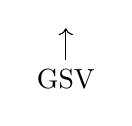
\begin{tikzpicture}
                \node[below] (A) at (0, 0) {GSV};
                \draw[->] (A) to (0, 0.4);
            \end{tikzpicture}
        }}{\leq} A(n, d)
        \underset{\mathclap{
            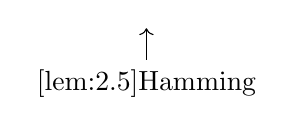
\begin{tikzpicture}
                \node[below] (A) at (0, 0) {\hyperref[lem:2.5]{Hamming}};
                \draw[->] (A) to (0, 0.4);
            \end{tikzpicture}
        }}{\leq}
        \frac{2^n}{V(n, \floor{\frac{n-1}{2}})}
    \end{equation*}
    % label the inequalities - GSV on left, Hamming on right
\end{nprop}
\begin{proof}
    Let $C$ be a code of length $n$ and minimum distance $d$ of largest possible size.
    Then $\nexists x \in \mathbb{F}_2^n$ such that $d(x, c) \geq d \quad \forall c \in C$, otherwise we would replace $C$ with $C \cup \{x\}$
    \begin{align*}
        \implies \mathbb{F}_2^n &\subseteq \bigcup_{c \in C}B(c, d-1) \\
        \implies 2^n &\leq \abs{C} V(n, d-1) \\
        \implies \abs{C} &\geq \frac{2^n}{V(n, d-1)}. \qedhere
    \end{align*}
\end{proof}
\begin{eg}
    Take $n=10$, $d=3$.
    \begin{align*}
        V(n, 1) &= 1 + 10 = 11 \\
        V(n, 2) &= 1 + 10 + \binom{10}{2} = 56
    \end{align*}
    \Cref{prop:2.6} gives $\frac{2^{10}}{56} \leq A(10, 3) \leq \frac{2^{10}}{11}$, so $19 \leq A(10, 3) \leq 93$. The exact value $A(10, 3) = 72$ was only found in 1999.
\end{eg}
There exist asymptotic versions of the \nameref{prop:2.6} and \nameref{lem:2.5}.
Let
\begin{equation*}\alpha(\delta) = \limsup \frac{1}{n} \log A(n, \delta n), \quad 0 \leq \delta \leq 1.\end{equation*}
\begin{notation}
    $H(\delta) = -\delta \log \delta - (1-\delta) \log (1-\delta)$.
\end{notation}
The asymptotic GSV says
\begin{equation*}
    \alpha(\delta) \geq 1 - H(\delta) \quad \text{for } 0 <\delta < \frac{1}{2}
\end{equation*}
while the asymptotic Hamming bound says
\begin{equation*}
    \alpha(\delta) \leq 1 - H\left(\frac{\delta}{2}\right).
\end{equation*}
We prove the asymptotic GSV bound
\begin{nprop}\label{prop:2.7}
    Let $0 < \delta < \frac{1}{2}$. Then
    \begin{enumerate}[label=(\roman*)]
        \item $\log V(n, \floor{n \delta}) \leq n H(\delta)$
        \item $\frac{\log A(n, \floor{n \delta})}{n} \geq 1 - H(\delta)$
    \end{enumerate}
\end{nprop}
\begin{proof}[Proof (i) $\Rightarrow$ (ii)]
    The \nameref{prop:2.6} gives
    \begin{align*}
        A(n, \floor{n \delta}) &\geq \frac{2^n}{V(n, \floor{n \delta} - 1)} \\
                               &\geq \frac{2^n}{V(n, \floor{n \delta})} \\
        \implies \log A(n, \floor{n \delta}) &\geq n - \log V(n, \floor{n \delta})\\
                                             &\geq n - n H(\delta) \qquad \text{by (i)} \\
        \implies \frac{\log A(n, \floor{n\delta})}{n} &\geq 1 - H(\delta) \qedhere
    \end{align*}
\end{proof}
\begin{proof}[Proof of (i)]
    \begin{align*}
        1 = (\delta + (1-\delta))^n &= \sum_{i=0}^n \binom{n}{i}\delta^i (1-\delta)^{n-i} \\
                                    &\geq \sum_{i=0}^{\floor{n \delta}} \binom{n}{i} \delta^i (1 - \delta)^{n-i} \\
                                    &= (1-\delta)^n \sum_{i=0}^{\floor{n\delta}} \binom{n}{i} \left(\frac{\delta}{1 - \delta}\right)^i\\
                                    &\geq (1-\delta)^n \sum_{i = 0}^{\floor{n \delta}} \binom{n}{i} \left(\frac{\delta}{1-\delta}\right)^{n\delta}\\
        1&\geq \delta^{n \delta} (1-\delta)^{n(1-\delta)} V(n, \floor{n\delta}) \\
        \implies 0 &\geq n(\delta \log \delta + (1-\delta) \log (1-\delta)) + \log V(n, \floor{n \delta}) \\
        \implies \log V(n, \floor{n \delta}) &\leq n H(\delta). \qedhere
    \end{align*}
\end{proof}
\subsection{Channel Capacity}
Let $\abs{\Sigma} = q$. A code of length $n$ is a subset of $\Sigma^n$ (usually we take $q=2$).

A code is used to send messages through a \hyperlink{def:dmc}{discrete memoryless channel} with $q$ input letters.
For each code a decoding rule is chosen.

\begin{defi}[Maximum error probability]\hypertarget{def:ehat}
    The \textbf{maximum error probability} is
\begin{equation*}
    \hat{e}(C) = \max_{c \in C} \Prob(\text{error} \mid c \text{ sent}).
\end{equation*}
\end{defi}
\begin{defi}[Reliable transmission]\hypertarget{def:relTrans}
    A channel can transmit \textbf{reliably at rate $R$} if there exists a sequence of codes $C_1, C_2, \dotsc$ where $C_n$ is a code of length $n$ and size $\floor{2^{nR}}$ such that
    \begin{equation*}
        \hyperlink{def:ehat}{\hat{e}(C_n)} \to 0 \text{ as } n \to \infty.
    \end{equation*}
\end{defi}
\begin{defi}
    The (operational) \textbf{channel capacity} is the supremum over all \hyperlink{def:relTrans}{reliable transmission} rates.
\end{defi}

% Lecture 9
\begin{nlemma}\label{lem:2.8}
    Let $\epsilon > 0$. A \hyperlink{def:bsc}{BSC} with error probability $p$ is used to send $n$ digits. Then
    \begin{equation*}
        \Prob(\text{BSC makes} \geq n(p + \epsilon) \text{ errors}) \to 0 \text{ as } n \to \infty.
    \end{equation*}
\end{nlemma}
\begin{proof}
    Let
    \begin{equation*}
        \mu_i =
        \begin{cases*}
            1 & if digit mistransmitted \\
            0 & otherwise
        \end{cases*}
    \end{equation*}
    $\mu_1, \mu_2, \mu_3, \dotsc$ are i.i.d.\ random variables.
    \begin{align*}
        \begin{rcases}
            \Prob(\mu_i = 1) = p \\
            \Prob(\mu_i = 0) = 1-p
        \end{rcases}
        \implies \Exp(\mu_i) &= p \\
        \Prob(\text{BSC makes} \geq n(p + \epsilon) \text{ errors}) &= \Prob(\sum_{i=1}^n \mu_i \geq n(p + \epsilon)) \\
                                                                    &\leq \Prob(\abs{\frac{1}{n} \sum \mu_i - p} \geq \epsilon)
    \end{align*}
    This $\to 0$ as $n \to \infty$ by \hyperlink{def:wlln}{WLLN}.
\end{proof}
\begin{remark}
    $\sum_{i=1}^n \mu_i$ is a binomial random variable with parameters $n$ and $p$.
\end{remark}
\begin{nprop}\label{prop:2.9}
\end{nprop}
% Lecture 10

% lecture 12
\begin{nlemma}
    Let $P \subset \mathbb{F}_2^n$ be a subset. Then $C = \set{x \in \mathbb{F}_2^n | p \cdot x = 0 \quad \forall p \in P}$ is a linear code.
\end{nlemma}
\begin{proof}
    \leavevmode
    \begin{enumerate}[label=(\roman*)]
        \item $0 \in C$ since $p \cdot 0 = 0$ $\forall p \in P$
        \item If $x, y \in C$, then $p \cdot (x+y) = p \cdot x + p \cdot y = 0 \implies x + y \in C$.
    \end{enumerate}
\end{proof}
$P$ is called a set of \textbf{parity checks} and $C$ is a \textbf{parity check code}.
\begin{defi}
    Let $C \subset \mathbb{F}_2^n$ be a linear code. The \textbf{dual code} is $C^\perp = \set{x \in \mathbb{F}_2^m | x \cdot y = 0 \quad \forall y \in C}$.
\end{defi}
This is a code by \cref{lem:2.18}.
\begin{nlemma}
    $\dim C + \dim C^\perp = n$.
\end{nlemma}
Warning: we can have $C \cap C^\perp \neq =\{0\}$.

\begin{proof}
    $V = \mathbb{F}_2^n$, $V^* = \{\text{linear maps: }V \to \mathbb{F}_2\}$. Consider
    \begin{align*}
        \phi : V &\longrightarrow V^* \\
        x &\longmapsto \theta_x \quad \text{where} \theta_x : y \longmapsto x \cdot y.
    \end{align*}
    $\phi$ is a linear map. SUppose $x \in \ker \phi$, then $x \cdot y = 0$ $\forall y \in V$.
    Taking $y = e_i (0, \dotsc, 0, 1, 0, \dotsc, 0)$ (with 1 in the $i$th place) gives $x_i = 0$. So $\ker \phi = \{0\}$.
    Since $\dim V = \dim V^*$, it follows that $\phi$ is an isomorphism.
    Thus
    \begin{align*}
        \theta(C^\perp) &= \set{\theta \in V^* | \theta(x) = 0 \ \forall x \in C} \\
                        &= \text{`annihilator of C'} = C^\circ
    \end{align*}
    so $\dim C + \dim \phi(C^\perp) = \dim V$, and $\dim C + \dim C^\perp = n$.
\end{proof}
\begin{cor}
    $(C^\perp)^\perp = C$ for any linear code $C$. In particular, any linear code is a parity check code.
\end{cor}
\begin{proof}
    Let $x \in C$. Then $x \cdot y = 0$ $\forall y \in C^\perp$, so $x \in (C^\perp)^\perp$, i.e.\ $C \subseteq (C^\perp)^\perp$.
    By \cref{lemma:2.19} (twice), $\dim (C^\perp)^\perp = dim C$, so $C = (C^\perp)^\perp$.
\end{proof}
\begin{defi}
    Let $C$ be a $(n, k)$ linear code.
    \begin{enumerate}[label=(\roman*)]
        \item A \textbf{generator matrix} for $C$ is a $k \times n$ matrix whose rows are a basis for $C$.
        \item A \textbf{parity check matrix} for $C$ is a generator matrix for $C^\perp$. It is a $(n-k) \times n$ matrix.
    \end{enumerate}
\end{defi}
\begin{nlemma}
    Every $(n, k)$ linear code is equivalent to  a linear code with generator matrix $\left( \begin{array}{c|c} I_k & B \end{array}\right)$.
\end{nlemma}
\begin{proof}
    We can perform row operations:
    \begin{itemize}
        \item swap 2 rows
        \item add one row to another
    \end{itemize}
    (multiplying by a scalar is not useful in $\mathbb{F}_2$).
    By Gaussian elimination, we get $G$, the generator matrix in row echelon form, e.g.\


    Permuting the columns of $G$ gives an equivalent code, i.e.\ $l(i) = i$ $1 \leq i \leq k$, i.e.\
    \begin{equation*}
        G =
        \left(
            \begin{array}{c c | c}
                1 & *  \\
            \end{array}
        \right)
    \end{equation*}
\end{proof}
\end{document}
